\documentclass[a4paper,11pt]{article}
\usepackage[T1]{fontenc}
\usepackage[utf8]{inputenc}
\usepackage[english]{babel}
\usepackage{amsmath,amssymb,mathtools}
\usepackage[margin=2.2cm]{geometry}
\usepackage{xcolor,tikz}
\usepackage[most]{tcolorbox}
\setlength{\parindent}{0pt}
\setlength{\parskip}{4pt}
\allowdisplaybreaks
\providecommand{\explainmode}{0}
\newif\ifexplain
\ifnum\explainmode=1 \explaintrue\fi
\newcommand{\aufgabe}[1]{\section*{Exercise #1}}
\newcommand{\angabe}[1]{\textit{#1}\par\smallskip}
\newcommand{\teil}[1]{\subsection*{#1}}
\newcommand{\why}[1]{\text{\small\color{black!65}#1}}
\newtcolorbox{erklbox}{colback=blue!4,colframe=blue!40,breakable,boxrule=0.5pt,title={Erklärung}}
\newcommand{\explain}[1]{\ifexplain\begin{erklbox}#1\end{erklbox}\fi}
\newcommand{\explainfig}[1]{\ifexplain\begin{center}#1\end{center}\fi}
\begin{document}
\begin{center}
{\Large Exercise sheet 5}\\
Linear Optimization (311.160), WS 2026/27\\
Raphael Bleier \qquad 9 November 2026
\end{center}
\explain{Ein Simplex-Schritt tauscht eine Basisvariable gegen eine Nichtbasisvariable. Die eintretende Variable hat positive reduzierte Kosten, die austretende bestimmt der Quotiententest. Sind danach alle reduzierten Kosten höchstens null, ist die Basislösung optimal. Auf diesem Blatt gibt es davon zwei, weil am Optimum eine reduzierte Kosten null bleibt und ein positiver Schritt noch zulässig ist. Kurz: zwei Ecken, ein Wert.}

\aufgabe{5.1}
\angabe{Maximize $x_1+x_2$ subject to $2x_1-x_2\leq 16$, $-x_1+x_2\leq 5$, $x_1+x_2\leq 10$ and $x\geq 0$.
1. Determine the optimal solution using the simplex method.
2. Show that the obtained solution is not unique by performing a different pivot at the beginning.
3. Solve the problem graphically and formulate a general criterion for detecting when an optimal solution is not unique.}
\explain{Die Zielfunktion steigt in beide Achsenrichtungen gleich stark. Deshalb haben $x_1$ und $x_2$ im Startdictionary dieselben reduzierten Kosten. Welche wir zuerst wählen, ist beides ein gültiger Simplex-Schritt. Die beiden Wege enden an den Endpunkten derselben optimalen Kante. Beide zählen.}

\teil{1. Slack form and the first simplex path}
Introduce nonnegative slacks $x_3,x_4,x_5$:
\begin{align*}
2x_1-x_2+x_3&=16&&\why{first inequality}\\
-x_1+x_2+x_4&=5&&\why{second inequality}\\
x_1+x_2+x_5&=10&&\why{third inequality}\\
z&=x_1+x_2&&\why{objective}
\end{align*}
The initial basis is $B=(3,4,5)$, with nonbasis $N=(1,2)$. Setting $x_1=x_2=0$ gives
\begin{align*}
x_3&=16&&\why{first equation at $x_N=0$}\\
x_4&=5&&\why{second equation}\\
x_5&=10&&\why{third equation}
\end{align*}
All three values are nonnegative, so the basic solution is feasible.
\explain{Die Schlupfvariable misst, wie viel bis zur Schranke fehlt. Am Nullpunkt sind alle drei Schranken noch nicht aktiv, deshalb sind die Schlupfwerte genau die rechten Seiten. Das ist die zulässige Startbasis für den Simplex.}
Solve the slacks for the basic variables:
\begin{align*}
x_3&=16-2x_1+x_2&&\why{move $2x_1-x_2$}\\
x_4&=5+x_1-x_2&&\why{move $-x_1+x_2$}\\
x_5&=10-x_1-x_2&&\why{move $x_1+x_2$}\\
z&=0+x_1+x_2&&\why{objective, constant term is $0$}
\end{align*}
The reduced costs of $(x_1,x_2)$ are $(1,1)$. Both are positive. The largest value occurs twice. The tie is broken by the smaller original index, so $x_1$ enters. This is the same rule as \texttt{numpy.argmax} on the ordered nonbasis.
\explain{Positive reduzierte Kosten heißen: die Zielfunktion wird größer, wenn wir diese Nichtbasisvariable erhöhen und die anderen bei null lassen. Hier bringen $x_1$ und $x_2$ denselben Zuwachs pro Einheit. Die Indexregel macht den ersten Lauf eindeutig, ohne eine der beiden Richtungen zu verbieten.}
In the dictionary $x_B=\overline b-\overline A x_N$, the column of $x_1$ is $(2,-1,1)^T$. Only positive entries can drive a basic variable down to zero:
\begin{align*}
\frac{16}{2}&=8&&\why{ratio for $x_3$}\\
\frac{10}{1}&=10&&\why{ratio for $x_5$}\\
8&<10&&\why{compare the two ratios}
\end{align*}
The coefficient of $x_1$ in the $x_4$ row is $-1$, so $x_4$ increases and does not limit the step. The leaving variable is $x_3$, with step length $8$.
\begin{align*}
x_3&=16-2x_1+x_2&&\why{dictionary row}\\
2x_1&=16-x_3+x_2&&\why{add $2x_1$, subtract $x_3$}\\
x_1&=8-\tfrac12 x_3+\tfrac12 x_2&&\why{divide by $2$}
\end{align*}
Substitute into the remaining rows:
\begin{align*}
x_4&=5+x_1-x_2&&\why{old row}\\
&=5+\bigl(8-\tfrac12 x_3+\tfrac12 x_2\bigr)-x_2&&\why{substitute $x_1$}\\
&=5+8-\tfrac12 x_3+\tfrac12 x_2-x_2&&\why{distribute}\\
&=13-\tfrac12 x_3+\tfrac12 x_2-x_2&&\why{add $5+8$}\\
&=13-\tfrac12 x_3-\tfrac12 x_2&&\why{$\tfrac12 x_2-x_2=-\tfrac12 x_2$}\\
x_5&=10-x_1-x_2&&\why{old row}\\
&=10-\bigl(8-\tfrac12 x_3+\tfrac12 x_2\bigr)-x_2&&\why{substitute $x_1$}\\
&=10-8+\tfrac12 x_3-\tfrac12 x_2-x_2&&\why{distribute the minus}\\
&=2+\tfrac12 x_3-\tfrac12 x_2-x_2&&\why{subtract}\\
&=2+\tfrac12 x_3-\tfrac32 x_2&&\why{collect $x_2$}\\
z&=x_1+x_2&&\why{objective}\\
&=8-\tfrac12 x_3+\tfrac12 x_2+x_2&&\why{substitute $x_1$}\\
&=8-\tfrac12 x_3+\tfrac32 x_2&&\why{collect $x_2$}
\end{align*}
With $x_3=x_2=0$ the new basic solution is $(x_1,x_2,x_3,x_4,x_5)=(8,0,0,13,2)$ and $z=8$. The reduced cost of $x_2$ is $\tfrac32>0$, so the dictionary is not optimal. $x_2$ enters.
\explain{Der erste Schritt läuft auf der $x_1$-Achse, bis die erste Nebenbedingung aktiv wird. $x_4$ und $x_5$ bleiben positiv. $x_2$ hat danach immer noch positive reduzierte Kosten, also lohnt ein zweiter Pivot. Noch nicht optimal.}
The column of $x_2$ decreases $x_4$ at rate $\tfrac12$ and $x_5$ at rate $\tfrac32$. The coefficient in the $x_1$ row is $-\tfrac12$, so $x_1$ increases.
\begin{align*}
\frac{13}{1/2}&=26&&\why{ratio for $x_4$}\\
\frac{2}{3/2}&=\tfrac43&&\why{ratio for $x_5$}\\
\tfrac43&<26&&\why{compare the ratios}
\end{align*}
Thus $x_5$ leaves, with step length $\tfrac43$.
\begin{align*}
x_5&=2+\tfrac12 x_3-\tfrac32 x_2&&\why{dictionary row}\\
\tfrac32 x_2&=2+\tfrac12 x_3-x_5&&\why{add $\tfrac32 x_2$, subtract $x_5$}\\
x_2&=\tfrac43+\tfrac13 x_3-\tfrac23 x_5&&\why{divide by $\tfrac32$}
\end{align*}
\begin{align*}
x_1&=8-\tfrac12 x_3+\tfrac12 x_2&&\why{old row}\\
&=8-\tfrac12 x_3+\tfrac12\bigl(\tfrac43+\tfrac13 x_3-\tfrac23 x_5\bigr)&&\why{substitute $x_2$}\\
&=8-\tfrac12 x_3+\tfrac23+\tfrac16 x_3-\tfrac13 x_5&&\why{distribute $\tfrac12$}\\
&=\tfrac{26}{3}-\tfrac12 x_3+\tfrac16 x_3-\tfrac13 x_5&&\why{$8+\tfrac23=\tfrac{24}{3}+\tfrac{2}{3}$}\\
&=\tfrac{26}{3}-\tfrac13 x_3-\tfrac13 x_5&&\why{$\tfrac12-\tfrac16=\tfrac13$}\\
x_4&=13-\tfrac12 x_3-\tfrac12 x_2&&\why{old row}\\
&=13-\tfrac12 x_3-\tfrac12\bigl(\tfrac43+\tfrac13 x_3-\tfrac23 x_5\bigr)&&\why{substitute $x_2$}\\
&=13-\tfrac12 x_3-\tfrac23-\tfrac16 x_3+\tfrac13 x_5&&\why{distribute}\\
&=\tfrac{37}{3}-\tfrac12 x_3-\tfrac16 x_3+\tfrac13 x_5&&\why{$13-\tfrac23=\tfrac{39}{3}-\tfrac{2}{3}$}\\
&=\tfrac{37}{3}-\tfrac23 x_3+\tfrac13 x_5&&\why{$\tfrac12+\tfrac16=\tfrac23$}\\
z&=8-\tfrac12 x_3+\tfrac32 x_2&&\why{old objective}\\
&=8-\tfrac12 x_3+\tfrac32\bigl(\tfrac43+\tfrac13 x_3-\tfrac23 x_5\bigr)&&\why{substitute $x_2$}\\
&=8-\tfrac12 x_3+2+\tfrac12 x_3-x_5&&\why{distribute $\tfrac32$}\\
&=10-\tfrac12 x_3+\tfrac12 x_3-x_5&&\why{add $8+2$}\\
&=10-x_5&&\why{the $x_3$ terms cancel}
\end{align*}
Set the new nonbasic variables $x_3=x_5=0$:
\begin{align*}
x_1&=\tfrac{26}{3}&&\why{constant term}\\
x_2&=\tfrac43&&\why{constant term}\\
x_4&=\tfrac{37}{3}&&\why{constant term}\\
z&=10&&\why{constant term}
\end{align*}
The reduced costs of $(x_3,x_5)$ are $(0,-1)$. Neither is positive, so this basic feasible solution is optimal for this pivot sequence.
\explain{Im neuen Dictionary steht vor $x_5$ eine negative reduzierte Kosten und vor $x_3$ eine null. Erhöhen wir eine Nichtbasisvariable mit negativer reduzierter Kosten, fällt $z$. Eine null ändert $z$ nicht. Für den ersten Lauf ist das der Abbruch: kein positiver Eintrag mehr. Die null ist der Hinweis, dass noch eine zweite optimale Ecke existieren kann. Das prüfen wir im zweiten Teil und an der Grafik.}
Probe in the original inequalities, with $x_1=\tfrac{26}{3}$ and $x_2=\tfrac43$:
\begin{align*}
2x_1-x_2&=2\cdot\tfrac{26}{3}-\tfrac43&&\why{substitute}\\
&=\tfrac{52}{3}-\tfrac43&&\why{multiply}\\
&=\tfrac{48}{3}&&\why{subtract}\\
&=16&&\why{divide}\\
-x_1+x_2&=-\tfrac{26}{3}+\tfrac43&&\why{substitute}\\
&=-\tfrac{22}{3}&&\why{add}\\
x_1+x_2&=\tfrac{26}{3}+\tfrac43&&\why{substitute}\\
&=\tfrac{30}{3}&&\why{add}\\
&=10&&\why{divide}\\
x_1+x_2&=10&&\why{objective at this point}
\end{align*}
So $2x_1-x_2=16\leq 16$, $-x_1+x_2=-\tfrac{22}{3}\leq 5$ and $x_1+x_2=10\leq 10$. Both coordinates are positive.
\[\boxed{x=\bigl(\tfrac{26}{3},\tfrac43\bigr)^T,\qquad z=10.}\]
\explain{Die Probe setzt den Punkt in die ursprünglichen Ungleichungen ein, nicht nur ins letzte Dictionary. Zwei Nebenbedingungen sind aktiv, die mittlere nicht. Das passt zu den Schlupfwerten $x_3=0$, $x_5=0$ und $x_4=\tfrac{37}{3}$.}

\teil{2. A different pivot at the beginning}
Start again from
\begin{align*}
x_3&=16-2x_1+x_2&&\why{initial dictionary}\\
x_4&=5+x_1-x_2&&\why{initial dictionary}\\
x_5&=10-x_1-x_2&&\why{initial dictionary}\\
z&=x_1+x_2&&\why{objective}
\end{align*}
Now let $x_2$ enter, although its reduced cost equals that of $x_1$. The column of $x_2$ is $(-1,1,1)^T$. The first entry is negative, so $x_3$ increases.
\begin{align*}
\frac{5}{1}&=5&&\why{ratio for $x_4$}\\
\frac{10}{1}&=10&&\why{ratio for $x_5$}\\
5&<10&&\why{compare the ratios}
\end{align*}
Hence $x_4$ leaves, with step length $5$.
\begin{align*}
x_4&=5+x_1-x_2&&\why{dictionary row}\\
x_2&=5+x_1-x_4&&\why{add $x_2$, subtract $x_4$}
\end{align*}
\begin{align*}
x_3&=16-2x_1+x_2&&\why{old row}\\
&=16-2x_1+(5+x_1-x_4)&&\why{substitute $x_2$}\\
&=16-2x_1+5+x_1-x_4&&\why{distribute}\\
&=21-2x_1+x_1-x_4&&\why{add $16+5$}\\
&=21-x_1-x_4&&\why{collect $x_1$}\\
x_5&=10-x_1-x_2&&\why{old row}\\
&=10-x_1-(5+x_1-x_4)&&\why{substitute $x_2$}\\
&=10-x_1-5-x_1+x_4&&\why{distribute the minus}\\
&=5-2x_1+x_4&&\why{collect terms}\\
z&=x_1+x_2&&\why{objective}\\
&=x_1+(5+x_1-x_4)&&\why{substitute $x_2$}\\
&=5+2x_1-x_4&&\why{collect $x_1$}
\end{align*}
With $x_1=x_4=0$ we have $(x_1,x_2)=(0,5)$, slacks $(21,0,5)$ and $z=5$. The reduced cost of $x_1$ is $2>0$, so $x_1$ enters. Its column decreases $x_3$ at rate $1$ and $x_5$ at rate $2$. The coefficient in the $x_2$ row is $-1$, so $x_2$ increases.
\begin{align*}
\frac{21}{1}&=21&&\why{ratio for $x_3$}\\
\frac{5}{2}&=\tfrac52&&\why{ratio for $x_5$}\\
\tfrac52&<21&&\why{compare the ratios}
\end{align*}
Thus $x_5$ leaves, with step length $\tfrac52$.
\begin{align*}
x_5&=5-2x_1+x_4&&\why{dictionary row}\\
2x_1&=5+x_4-x_5&&\why{add $2x_1$, subtract $x_5$}\\
x_1&=\tfrac52+\tfrac12 x_4-\tfrac12 x_5&&\why{divide by $2$}
\end{align*}
\begin{align*}
x_2&=5+x_1-x_4&&\why{old row}\\
&=5+\bigl(\tfrac52+\tfrac12 x_4-\tfrac12 x_5\bigr)-x_4&&\why{substitute $x_1$}\\
&=\tfrac{15}{2}+\tfrac12 x_4-\tfrac12 x_5-x_4&&\why{add $5+\tfrac52$}\\
&=\tfrac{15}{2}-\tfrac12 x_4-\tfrac12 x_5&&\why{$\tfrac12 x_4-x_4=-\tfrac12 x_4$}\\
x_3&=21-x_1-x_4&&\why{old row}\\
&=21-\bigl(\tfrac52+\tfrac12 x_4-\tfrac12 x_5\bigr)-x_4&&\why{substitute $x_1$}\\
&=\tfrac{37}{2}-\tfrac12 x_4+\tfrac12 x_5-x_4&&\why{$21-\tfrac52=\tfrac{42}{2}-\tfrac{5}{2}$}\\
&=\tfrac{37}{2}-\tfrac32 x_4+\tfrac12 x_5&&\why{collect $x_4$}\\
z&=5+2x_1-x_4&&\why{old objective}\\
&=5+2\bigl(\tfrac52+\tfrac12 x_4-\tfrac12 x_5\bigr)-x_4&&\why{substitute $x_1$}\\
&=5+5+x_4-x_5-x_4&&\why{distribute}\\
&=10-x_5&&\why{the $x_4$ terms cancel}
\end{align*}
Set $x_4=x_5=0$:
\begin{align*}
x_1&=\tfrac52&&\why{constant term}\\
x_2&=\tfrac{15}{2}&&\why{constant term}\\
x_3&=\tfrac{37}{2}&&\why{constant term}\\
z&=10&&\why{constant term}
\end{align*}
The reduced costs of $(x_5,x_4)$ are $(-1,0)$. No reduced cost is positive, so this point is also optimal. It is not the point from part 1:
\begin{align*}
\tfrac{26}{3}-\tfrac52&=\tfrac{52}{6}-\tfrac{15}{6}&&\why{common denominator}\\
&=\tfrac{37}{6}&&\why{subtract}\\
\tfrac{37}{6}&\neq 0&&\why{the first coordinates differ}
\end{align*}
Both objective values equal $10$. Therefore the optimal solution obtained in part 1 is not unique.
\explain{Der andere erste Pivot läuft zuerst die $x_2$-Achse hinauf bis $(0,5)$ und dann entlang $-x_1+x_2=5$ bis zur dritten Nebenbedingung. Wieder ist $z=10$, aber die Koordinaten sind andere. Genau das verlangt Teil 2: nicht eine andere Basis desselben Punkts, sondern ein anderer Punkt. Nicht dieselbe Ecke.}
Probe with $x_1=\tfrac52$ and $x_2=\tfrac{15}{2}$:
\begin{align*}
2x_1-x_2&=2\cdot\tfrac52-\tfrac{15}{2}&&\why{substitute}\\
&=5-\tfrac{15}{2}&&\why{multiply}\\
&=-\tfrac52&&\why{subtract}\\
-x_1+x_2&=-\tfrac52+\tfrac{15}{2}&&\why{substitute}\\
&=\tfrac{10}{2}&&\why{add}\\
&=5&&\why{divide}\\
x_1+x_2&=\tfrac52+\tfrac{15}{2}&&\why{substitute}\\
&=10&&\why{add}
\end{align*}
So $2x_1-x_2=-\tfrac52\leq 16$, $-x_1+x_2=5\leq 5$ and $x_1+x_2=10\leq 10$. Both coordinates are positive.
\[\boxed{x=\bigl(\tfrac52,\tfrac{15}{2}\bigr)^T,\qquad z=10,\quad\text{different from part 1.}}\]

\teil{3. Graphical solution and the uniqueness criterion}
Rewrite the inequalities as bounds on $x_2$:
\begin{align*}
x_2&\geq 2x_1-16&&\why{first inequality, add $x_2$, subtract $16$}\\
x_2&\leq x_1+5&&\why{second inequality, add $x_1$}\\
x_2&\leq 10-x_1&&\why{third inequality, subtract $x_1$}\\
x_1&\geq 0&&\why{sign restriction}\\
x_2&\geq 0&&\why{sign restriction}
\end{align*}
The binding pairs that can produce a vertex are the axis intersections and the pairwise intersections of the three lines. Compute them one pair at a time.
\begin{align*}
2x_1&=16&&\why{$x_2=0$ in the first equation}\\
x_1&=8&&\why{divide by $2$}
\end{align*}
The point $(8,0)$ satisfies $-8\leq 5$ and $8\leq 10$.
\begin{align*}
x_2&=5&&\why{$x_1=0$ in the second equation}
\end{align*}
The point $(0,5)$ satisfies $-5\leq 16$ and $5\leq 10$.
\begin{align*}
x_1+5&=10-x_1&&\why{second and third lines}\\
2x_1&=5&&\why{add $x_1$, subtract $5$}\\
x_1&=\tfrac52&&\why{divide by $2$}\\
x_2&=10-\tfrac52&&\why{third line}\\
&=\tfrac{15}{2}&&\why{subtract}
\end{align*}
Check the first inequality at this intersection:
\begin{align*}
2\cdot\tfrac52-\tfrac{15}{2}&=-\tfrac52&&\why{same calculation as the probe}\\
-\tfrac52&\leq 16&&\why{compare with the bound}
\end{align*}
Next, the first and third lines:
\begin{align*}
2x_1-(10-x_1)&=16&&\why{substitute $x_2=10-x_1$}\\
2x_1-10+x_1&=16&&\why{distribute}\\
3x_1&=26&&\why{add $10$}\\
x_1&=\tfrac{26}{3}&&\why{divide by $3$}\\
x_2&=10-\tfrac{26}{3}&&\why{third line}\\
&=\tfrac43&&\why{subtract}
\end{align*}
Check the second inequality:
\begin{align*}
-\tfrac{26}{3}+\tfrac43&=-\tfrac{22}{3}&&\why{add}\\
-\tfrac{22}{3}&\leq 5&&\why{compare with the bound}
\end{align*}
The remaining line pairs miss the feasible region. For the first and second lines,
\begin{align*}
2x_1-(x_1+5)&=16&&\why{substitute $x_2=x_1+5$}\\
x_1-5&=16&&\why{distribute}\\
x_1&=21&&\why{add $5$}\\
x_2&=26&&\why{$21+5$}\\
x_1+x_2&=47&&\why{add}\\
47&>10&&\why{violates the third inequality}
\end{align*}
For the first line and $x_1=0$, the value $x_2=-16$ is negative. The origin is the remaining feasible corner. The feasible vertices and their objective values are therefore
\begin{align*}
z(0,0)&=0&&\why{sum of coordinates}\\
z(8,0)&=8&&\why{sum of coordinates}\\
z(0,5)&=5&&\why{sum of coordinates}\\
z\bigl(\tfrac{26}{3},\tfrac43\bigr)&=10&&\why{sum, already checked}\\
z\bigl(\tfrac52,\tfrac{15}{2}\bigr)&=10&&\why{sum, already checked}
\end{align*}
The largest value is $10$, attained at two vertices. A level line of the objective is $x_2=-x_1+t$. Its slope is $-1$, the same slope as $x_1+x_2=10$. Shifting the line upward in the objective direction, the last contact with the feasible polygon is that whole edge, not a single vertex.
\begin{center}
% grafik-verlangt
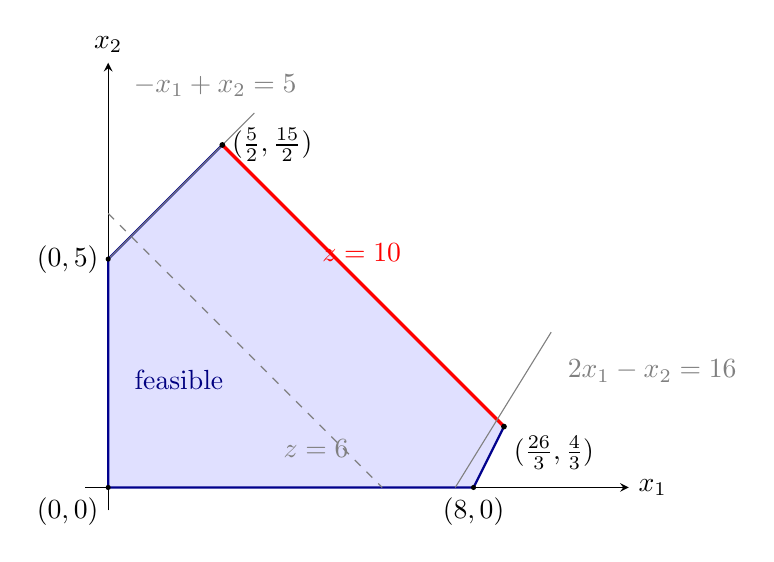
\begin{tikzpicture}[scale=0.58,>=stealth]
  \draw[->] (-0.5,0) -- (11.4,0) node[right] {$x_1$};
  \draw[->] (0,-0.5) -- (0,9.3) node[above] {$x_2$};
  \fill[blue!12] (0,0) -- (8,0) -- ({26/3},{4/3}) -- (2.5,7.5) -- (0,5) -- cycle;
  \draw[thick,blue!55!black] (0,0) -- (8,0) -- ({26/3},{4/3}) -- (2.5,7.5) -- (0,5) -- cycle;
  \draw[red,very thick] (2.5,7.5) -- ({26/3},{4/3});
  \draw[gray,dashed] (0,6) -- (6,0);
  \draw[gray] (7.6,0) -- (9.7,3.4);
  \draw[gray] (0,5) -- (3.2,8.2);
  \fill (0,0) circle (1.6pt) node[below left] {$(0,0)$};
  \fill (8,0) circle (1.6pt) node[below] {$(8,0)$};
  \fill ({26/3},{4/3}) circle (1.8pt) node[below right] {$(\frac{26}{3},\frac{4}{3})$};
  \fill (2.5,7.5) circle (1.8pt) node[right] {$(\frac{5}{2},\frac{15}{2})$};
  \fill (0,5) circle (1.6pt) node[left] {$(0,5)$};
  \node[red] at (5.55,5.15) {$z=10$};
  \node[gray] at (4.55,0.85) {$z=6$};
  \node[gray,anchor=west] at (9.85,2.55) {$2x_1-x_2=16$};
  \node[gray,anchor=south west] at (0.35,8.35) {$-x_1+x_2=5$};
  \node[blue!50!black] at (1.55,2.35) {feasible};
\end{tikzpicture}
\end{center}
The two optimal basic solutions are the endpoints of this edge. The feasible region is convex, and the objective is linear. For $\lambda\in[0,1]$,
\begin{align*}
x(\lambda)&=\lambda\bigl(\tfrac{26}{3},\tfrac43\bigr)^T+(1-\lambda)\bigl(\tfrac52,\tfrac{15}{2}\bigr)^T&&\why{segment between the endpoints}\\
z\bigl(x(\lambda)\bigr)&=\lambda\cdot 10+(1-\lambda)\cdot 10&&\why{both endpoints have objective $10$}\\
&=10&&\why{the $\lambda$ terms cancel}
\end{align*}
Every point of the segment is feasible and optimal. One explicit midpoint, $\lambda=\tfrac12$, is
\begin{align*}
x_1&=\tfrac12\cdot\tfrac{26}{3}+\tfrac12\cdot\tfrac52&&\why{substitute $\lambda$}\\
&=\tfrac{13}{3}+\tfrac54&&\why{multiply}\\
&=\tfrac{52}{12}+\tfrac{15}{12}&&\why{common denominator}\\
&=\tfrac{67}{12}&&\why{add}\\
x_2&=\tfrac12\cdot\tfrac43+\tfrac12\cdot\tfrac{15}{2}&&\why{substitute $\lambda$}\\
&=\tfrac23+\tfrac{15}{4}&&\why{multiply}\\
&=\tfrac{8}{12}+\tfrac{45}{12}&&\why{common denominator}\\
&=\tfrac{53}{12}&&\why{add}\\
x_1+x_2&=\tfrac{67}{12}+\tfrac{53}{12}&&\why{add the coordinates}\\
&=10&&\why{sum of the numerators is $120$}
\end{align*}
The midpoint also satisfies the other two inequalities:
\begin{align*}
2x_1-x_2&=2\cdot\tfrac{67}{12}-\tfrac{53}{12}&&\why{substitute the midpoint}\\
&=\tfrac{134}{12}-\tfrac{53}{12}&&\why{multiply}\\
&=\tfrac{81}{12}&&\why{subtract}\\
&=\tfrac{27}{4}&&\why{divide by $3$}\\
-x_1+x_2&=-\tfrac{67}{12}+\tfrac{53}{12}&&\why{substitute}\\
&=-\tfrac{14}{12}&&\why{add}\\
&=-\tfrac{7}{6}&&\why{divide by $2$}
\end{align*}
So $2x_1-x_2=\tfrac{27}{4}\leq 16$ and $-x_1+x_2=-\tfrac{7}{6}\leq 5$.
\explain{Die gestrichelte Linie $z=6$ ist parallel zur optimalen Kante und schneidet das Gebiet noch innen. Schiebt man sie weiter, bleibt sie bis $z=10$ im Gebiet und liegt dann genau auf der Kante. Ein einzelner Eckpunkt wäre nur dann die einzige Lösung, wenn die Niveaulinie das Gebiet zuletzt in genau einem Punkt berührt.}
\explainfig{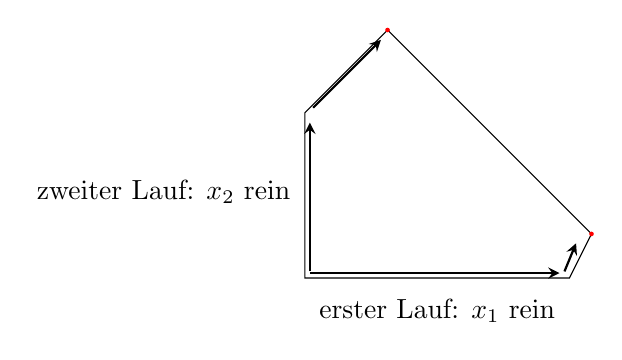
\begin{tikzpicture}[scale=0.42,>=stealth]
  \draw (0,0) -- (8,0) -- ({26/3},{4/3}) -- (2.5,7.5) -- (0,5) -- cycle;
  \draw[->,thick] (0.15,0.15) -- (7.7,0.15);
  \draw[->,thick] (7.85,0.2) -- (8.2,1.05);
  \draw[->,thick] (0.15,0.2) -- (0.15,4.7);
  \draw[->,thick] (0.25,5.15) -- (2.3,7.2);
  \node[below] at (4,-0.35) {erster Lauf: $x_1$ rein};
  \node[left] at (-0.15,2.6) {zweiter Lauf: $x_2$ rein};
  \fill[red] ({26/3},{4/3}) circle (2pt);
  \fill[red] (2.5,7.5) circle (2pt);
\end{tikzpicture}}
Criterion, for a maximization problem written as $z=\overline z+\overline c_N^T x_N$. If an optimal dictionary has $\overline c_j<0$ for every nonbasic index $j$, then every feasible increase of a nonbasic variable decreases $z$. The optimal solution is unique. If some nonbasic reduced cost is zero and the minimum-ratio test for that variable returns a positive step, pivoting on it produces a different optimal basic solution. The optimum is then not unique, and every convex combination of optimal solutions is optimal. A zero reduced cost whose ratio is zero only changes the basis at the same point. That alone does not show a second solution.
Graphically, in two variables, the optimal solution is not unique exactly when an optimal level line contains an edge of the feasible region. In this problem the level line $x_1+x_2=10$ is the third constraint, restricted to the segment between the two basic solutions above.
\[\boxed{\begin{aligned}
&x(\lambda)=\lambda\bigl(\tfrac{26}{3},\tfrac43\bigr)^T+(1-\lambda)\bigl(\tfrac52,\tfrac{15}{2}\bigr)^T,\ \lambda\in[0,1],\ z=10,\\
&\text{not unique iff an optimal dictionary has a zero reduced cost with positive step.}
\end{aligned}}\]
\explain{Die Dictionary-Regel gilt auch in höheren Dimensionen, nicht nur in der Zeichnung mit zwei Variablen. Strikt negative reduzierte Kosten schließen jede andere zulässige Verbesserung aus, nicht bloß eine andere Basis desselben Punkts. Eine reduzierte Kosten von null mit positivem Quotienten ist die Kante, die man in der Zeichnung sieht. Hier ist der Quotient positiv. Ist der Quotient null, bleibt man auf demselben Punkt. Das wäre Degeneration. Hier tritt sie nicht auf.}

\aufgabe{5.2}
\angabe{Consider $\max\, c^T x$ subject to $Ax\leq 0$ and $x\geq 0$. Show that either $x=0$ is optimal or the LP is unbounded.}
The zero vector is feasible:
\begin{align*}
A\cdot 0&=0&&\why{matrix times the zero vector}\\
0&\leq 0&&\why{the inequality $Ax\leq 0$ holds}\\
0&\geq 0&&\why{the sign restriction holds}\\
c^T\cdot 0&=0&&\why{objective at $x=0$}
\end{align*}
\explain{Die zulässige Menge ist ein Kegel mit Spitze im Ursprung. Jeder zulässige Punkt darf mit einer nichtnegativen Zahl gestreckt werden, ohne die Nebenbedingungen zu verlassen. Deshalb gibt es nur die beiden Fälle aus der Aufgabe.}
Either $c^T x\leq 0$ for every feasible $x$, or there exists a feasible $\hat x$ with $c^T\hat x>0$.
Case 1. Assume $c^T x\leq 0$ whenever $Ax\leq 0$ and $x\geq 0$. Then
\begin{align*}
c^T x&\leq 0&&\why{assumption of this case}\\
c^T x&\leq c^T\cdot 0&&\why{the right-hand side is the value at zero}
\end{align*}
for every feasible $x$. Therefore $x=0$ is optimal.
Case 2. Assume $\hat x$ is feasible and $c^T\hat x>0$. For every $t\geq 0$ set $x(t)=t\hat x$. Then
\begin{align*}
Ax(t)&=t\,A\hat x&&\why{factor $t$ out of the matrix product}\\
t\,A\hat x&\leq 0&&\why{$t\geq 0$ and $A\hat x\leq 0$}\\
x(t)&=t\hat x&&\why{definition of the ray}\\
t\hat x&\geq 0&&\why{$t\geq 0$ and $\hat x\geq 0$}
\end{align*}
so $x(t)$ is feasible. Its objective value is
\begin{align*}
c^T x(t)&=t\,c^T\hat x&&\why{factor $t$}\\
t\,c^T\hat x&\to\infty&&\why{$c^T\hat x>0$ and $t\to\infty$}
\end{align*}
The feasible values are not bounded above, so the LP is unbounded.
The two cases cover every $c$ and every $A$. A positive cost coefficient by itself is not the second case: the corresponding unit step must still satisfy $Ax\leq 0$.
\[\boxed{\text{Either }x=0\text{ is optimal, or the LP is unbounded.}}\]
\explain{Der häufige Fehlschluss ist, aus einem positiven $c_j$ sofort Unbeschränktheit zu lesen. Das stimmt nur, wenn die Spalte $A_{\cdot j}$ selbst keine positive Komponente hat, denn nur dann bleibt $t e_j$ zulässig. Hat die Spalte einen positiven Eintrag, blockiert diese Zeile schon jeden positiven Schritt, und $x=0$ kann trotzdem optimal sein. Der Beweis benutzt deshalb einen tatsächlich zulässigen Punkt mit positivem Wert und streckt genau diesen. Positives $c_j$ allein reicht nicht.}

\aufgabe{5.3}
\angabe{Complete \texttt{choose\_entering\_variable\_index} and \texttt{choose\_leaving\_variable\_index} from \texttt{Exercise\_05.py}. Together with \texttt{initial\_simplex\_dictionary} from sheet 4, test them on Example 2.2. Submit \texttt{LASTNAME\_sheet\_NUMBER.py} and \texttt{LASTNAME\_sheet\_NUMBER.pdf}.}
\teil{Entering variable}
The function reads \texttt{c\_bar\_N} and \texttt{N} from the dictionary of sheet 4. That dictionary stores $x_B=\overline b-\overline A x_N$ and $z=\overline z+\overline c_N^T x_N$, so a positive reduced cost is an improving direction for maximization. If no entry of \texttt{c\_bar\_N} exceeds $10^{-9}$, the function returns \texttt{None}. Otherwise it returns the original index in \texttt{N} at which \texttt{c\_bar\_N} is maximal. A tie keeps the first maximum, which is the earlier position in \texttt{N}.
\teil{Leaving variable}
Given the entering index, the function takes the matching column of \texttt{A\_bar}. Rows whose entry does not exceed $10^{-9}$ are ignored, because those basic variables do not decrease. If no row remains, the function returns \texttt{None}: the entering variable can increase without a bound from the current dictionary, and the LP is unbounded along that ray. Otherwise it returns the original index in \texttt{B} of the smallest ratio $\overline b_i/\overline A_{i,\mathrm{enter}}$. A tie keeps the first minimum in the current order of \texttt{B}.
\explain{Die Toleranz steht schon im Skelett. Sie verhindert, dass Rundungsrauschen eine fast null als Eintritts- oder Austrittskandidat zählt. Bei Gleichstand folgt der Code der Reihenfolge im Dictionary, nicht einer zusätzlichen Bland-Regel über alle Variablenindizes. Für Example 2.2 gibt es keinen Gleichstand.}
\teil{Test on Example 2.2}
Example 2.2 is $\max -x_1+2x_2+6x_3$ with
\begin{align*}
2x_1+3x_2+x_4&=10&&\why{first constraint of Example 2.2}\\
x_1+2x_3+x_5&=8&&\why{second constraint}\\
x_1+2x_2+x_3+x_6&=6&&\why{third constraint}
\end{align*}
and $x\geq 0$. The initial call uses the zero-based basis \texttt{[3, 4, 5]}. Sheet 4 already gives
\[\overline c_N=(-1,2,6)^T,\qquad N=(0,1,2),\qquad B=(3,4,5).\]
The unique maximum reduced cost is $6$, at position $2$ of $N$:
\begin{align*}
6&>2&&\why{compare the positive reduced costs}\\
6&>-1&&\why{compare with the remaining cost}
\end{align*}
so the entering index is $2$, the variable $x_3$. Its column in $\overline A$ is $(0,2,1)^T$.
\begin{align*}
\frac{8}{2}&=4&&\why{ratio in the $x_5$ row}\\
\frac{6}{1}&=6&&\why{ratio in the $x_6$ row}\\
4&<6&&\why{compare the ratios}
\end{align*}
The first row has coefficient $0$ and is skipped. The leaving index is $4$, the variable $x_5$. After this pivot the basic solution is $(0,0,4,10,0,2)^T$ with value $24$, as in Lecture 4. The completed file \texttt{Bleier\_sheet\_5.py} prints these two indices. \texttt{test\_sheet5.py} also checks an optimal dictionary, an unbounded column, both tie rules and the second lecture pivot from this point to $z=26$.
\[\boxed{\text{entering index }2\ (x_3),\qquad \text{leaving index }4\ (x_5).}\]
\explain{Im Dictionary steht das Minus vor $\overline A$, nicht in der gespeicherten Matrix. Der Quotiententest teilt deshalb $\overline b$ durch die positive Spalte von $\overline A$. Wer das Vorzeichen in die Matrix zieht, sucht die austretende Variable in der falschen Spalte. Die Indizes in Python sind um eins kleiner als die Variablennummern aus der Vorlesung. Eins weniger.}

\explain{Classroom task 5.1, nur als Lernzusatz. Der Startpunkt ist eine zulässige Basislösung, also ein Dictionary mit $\overline b\geq 0$. In der Schleife berechnen wir die reduzierten Kosten $\overline c_N=c_N-\overline A^T c_B$. Die gewünschte Eigenschaft ist $\overline c_N\leq 0$: keine Nichtbasisvariable kann die Zielfunktion noch erhöhen. Dann ist die aktuelle Basislösung optimal und wir stoppen. Sonst wählen wir eine Nichtbasisvariable mit positiver reduzierter Kosten. Die austretende Variable liefert der Quotiententest. Hat die Spalte keinen positiven Eintrag, ist das LP unbeschränkt. Gibt es beide Indizes, tauschen wir sie und schreiben das Dictionary neu. Dann von vorn. Das ist genau der Ablauf aus den beiden Läufen in Aufgabe 5.1 und aus dem Test von Example 2.2, nur ohne die konkreten Zahlen dieses Blatts.}
\end{document}
